\textbf{Ejemplo 1}\\

Una persona está pensando en construir un parqueadero, para tal fin toma en alquiler un lote por un plazo de 5 años. El costo de la construcción, incluidos los impuestos y las licencias, son del orden de  COP  15.000.000; se estima que los ingresos después de descontar el valor de los arriendos e impuestos, es decir, los ingresos netos, son del orden de  COP  5.000.000 los cuales crecerán cada año aproximadamente de acuerdo al índice de inflación que se estima en un 20\% período anual vencido. Si el inversionista gana normalmente en todos sus negocios un 35\% período anual vencido. ¿Es aconsejable este negocio?
\\

\textbf{Solución.}\\
%La tabla ira centrada
\begin{center}
	\renewcommand{\arraystretch}{1.5}% Margenes de las celdas
	%Creación de la cuadricula de 3 columnas
\begin{longtable}[H]{|c|c|c|}
		%Creamos una linea horizontal
\hline
		%Definimos el color de la primera fila
\rowcolor[HTML]{FFB183}

%%%%% INICIO ASIGNACIÓN PERÍODO FOCAL %%%%%%%
  %%%%%%%%%% INICIO TITULO
  %Lo que se hace aquí es mezclar las 3 columnas en una sola
  \multicolumn{3}{|c|}{\cellcolor[HTML]{FFB183}\textbf{1. Asignación período focal}}   \\ \hline
  %%%%%%%%%% FIN TITULO
  %%%%% INICIO DECLARACIÓN DE VARIABLES %%%%%%%
  \multicolumn{3}{|c|}{$pf = 0 pav$}   \\ \hline

%%%%%%%%%%% INICIO TITULO
\rowcolor[HTML]{FFB183}
\multicolumn{3}{|c|}{\cellcolor[HTML]{FFB183}\textbf{2. Declaración de variables}}    \\ \hline
%%%%%%%%%%% FIN TITULO
%%%%%%%%%%% INICIO MATEMÁTICAS

$i_{1} = 20\% pav$                                     & \multicolumn{2}{c|}{$ i_{2} = 35\% pav $} \\
$n = 5 pav \hspace{0.3cm} $	& \multicolumn{2}{c|}{$ \textbf{ingresos netos} =  COP  5.000.000 $} \\
$ \textbf{inversion inicial} =  COP  15.000.000 $	&	\multicolumn{2}{c|}{ $ $ } \\ \hline
%%%%%%%%%% FIN MATEMÁTICAS
		%%%%% INICIO FLUJO DE CAJA
\rowcolor[HTML]{FFB183}
\multicolumn{3}{|c|}{\cellcolor[HTML]{FFB183}\textbf{3. Diagrama de flujo de caja}} \\ \hline
		%Mezclamos 3 columnas y pondremos el dibujo
		%%%%%%%%%%%%% INSERCIÓN DE LA IMAGEN
		%Deberán descargar las imágenes respectivas del drive y pegarlas en la carpeta
		%n_capitulo/img/ejemplos/1/capitulo1ejemplo1.pdf  (el /1/ es el numero del ejemplo)
\multicolumn{3}{|c|}{ 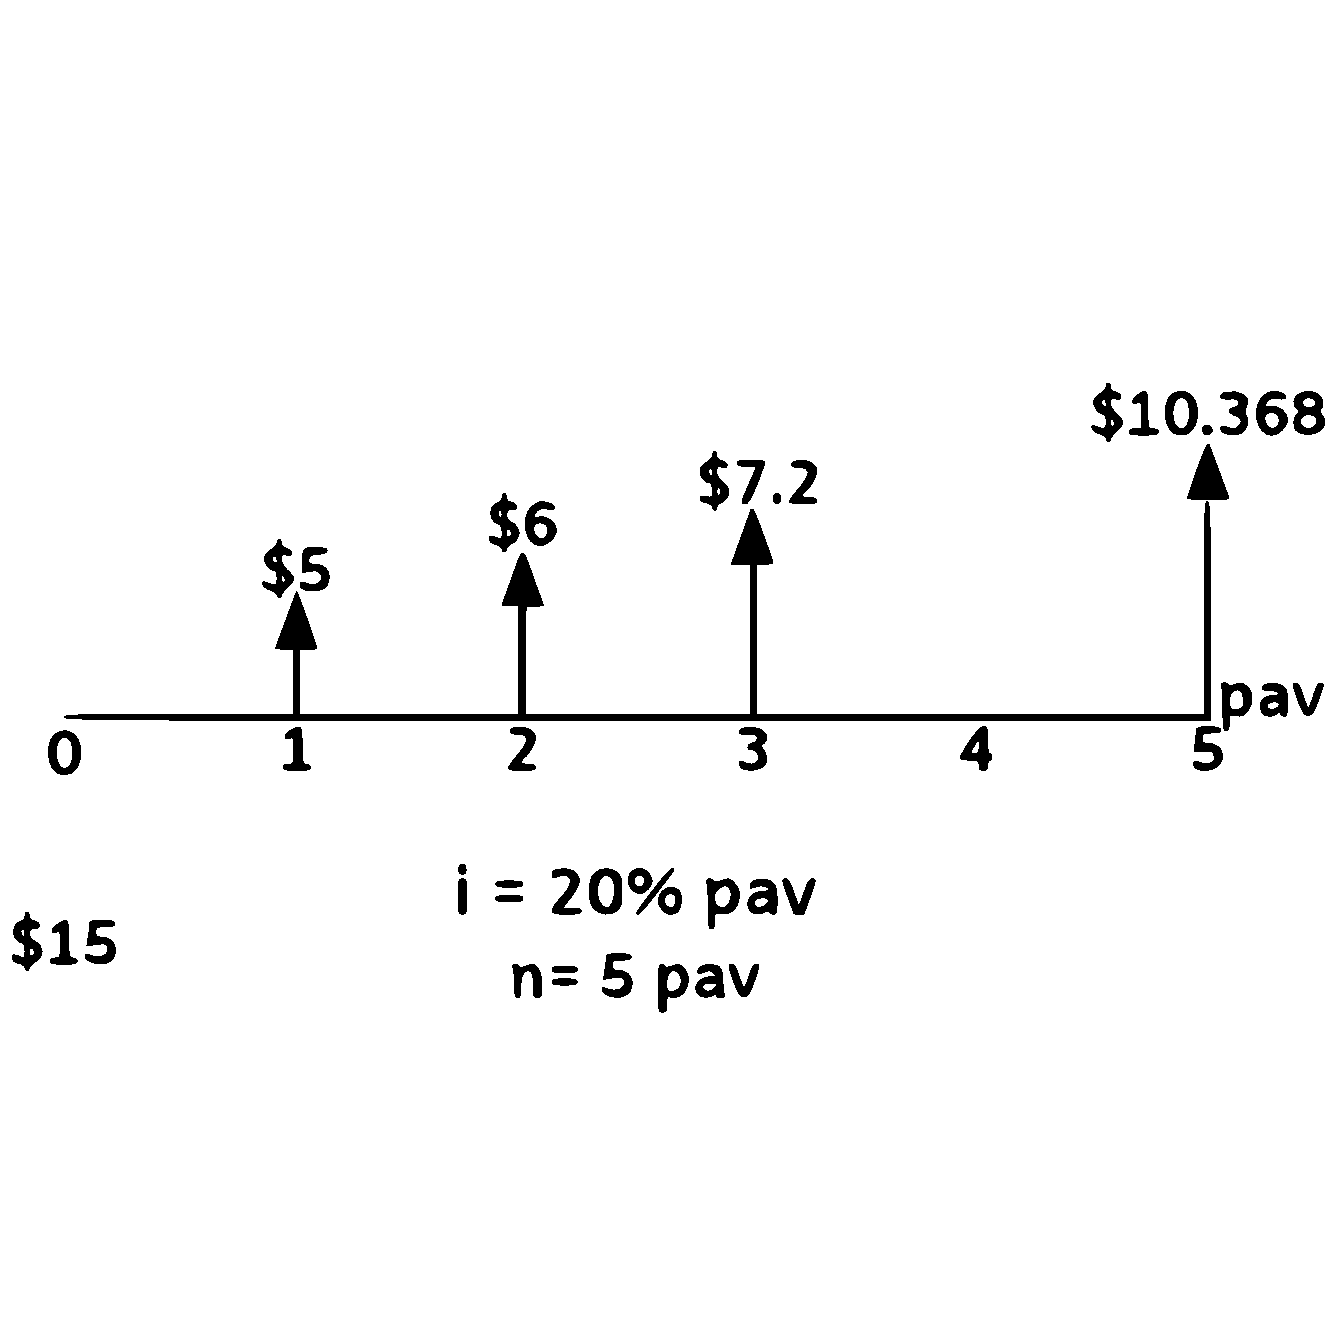
\includegraphics[scale=0.6, trim=-5 -5 -5 -5]{Graf3Cap11.pdf} }   
   \\ \hline
		%%%%%%%%%%%%% FIN INSERCIÓN DE IMAGEN
		%%%%%FIN FLUJO DE CAJA
		
		
		
		%%%%% INICIO DECLARACIÓN FORMULAS
		%%%%%%%%%%% INICIO TITULO
\rowcolor[HTML]{FFB183}
\multicolumn{3}{|c|}{\cellcolor[HTML]{FFB183}\textbf{4. Declaración de fórmulas}}    \\ \hline
		%%%%%%%%%%% FIN TITULO
		%%%%%%%%%%% INICIO MATEMÁTICAS
\multicolumn{3}{|c|} {$VPN =\sum F_{n}(1+i)^{-n} $ Valor presente neto.}   \\ \hline	
	
		%%%%%%%%%% FIN MATEMÁTICAS
		%%%%%% INICIO DESARROLLO MATEMÁTICO
\rowcolor[HTML]{FFB183}
		%%%%%%%%%%INICIO TITULO
\multicolumn{3}{|c|}{\cellcolor[HTML]{FFB183}\textbf{5. Desarrollo matemático}}       \\ \hline
		%%%%%%%%%% FIN TITULO
		%%%%%%%%%% INICIO MATEMÁTICAS
		\multicolumn{3}{|c|}{$VPN = -15+\frac{5[(1+0.2)^5(1+i)^{-5}-1]}{0.2-i}= COP  0  \textbf{ Valor presente neto.} $}  
		\\
		
		\multicolumn{3}{|c|}{$ 	VPN(30\%) = -15+\frac{[(1+0.2)^5(1+0.3)^{-5}-1]}{0.2-0.3}= COP  1.49115   \textbf{      Valor presente neto.} $}  
		\\
	
		\multicolumn{3}{|c|}{$ \frac{34-35}{34-X} = \frac{0.14476-(-0.1643)}{0.14476-0} \textbf{   Ecuación de valor} $}
		\\ \hline
				
		%%%%%%%%%% FIN MATEMÁTICAS
		%%%%%% FIN DESARROLLO MATEMÁTICO
		%%%%%% INICIO RESPUESTA
\rowcolor[HTML]{FFB183}
		%%%%%%%%%%INICIO TITULO
\multicolumn{3}{|c|}{\cellcolor[HTML]{FFB183}\textbf{6. Respuesta}}   \\ \hline
		%%%%%%%%%% FIN TITULO
		%%%%%%%%%% INICIO RESPUESTA MATEMÁTICA
		
\multicolumn{3}{|c|}{ $ X = 34.468\% pav$ }  \\ 
\multicolumn{3}{|c|}{ \textbf{No debe ser aceptada porque la TIR es inferior a la tasa del inversionista de 35\% pav,} }  \\ 
\multicolumn{3}{|c|}{ \textbf{para captar el interés del inversionista hay que ofrecer una tasa más alta,} }  \\ 
\multicolumn{3}{|c|}{ \textbf{y así acaparar su interés por el
proyecto, la denominada tasa mínima atractiva de retorno.} }  \\ 
\hline
		
		
		%%%%%%%%%% FIN MATEMÁTICAS
		%%%%%% FIN RESPUESTA
	\end{longtable}
	%Se crean dos lineas en blanco para que no quede el siguiente texto tan pegado
	%\newline \newline %USARLO SI CREES QUE ES NECESARIO
\end{center}
%%%%%%%%%%%%%%%%%%%%%%%%%%FIN EJERCICIO 1 %%%%%%%%%%%%%%%%%%%%%%%%%%%
